% Advanced NLP - Assignment 1 Report
% Formatting per the assignment brief: 12pt Times New Roman, 1-inch margins,
% maximum 6 pages excluding references and links.
%
% Compile from this directory (the figure paths are relative to it):
%   pdflatex Report.tex && pdflatex Report.tex
% Then copy Report.pdf into 2023111026_assignment1/.

\documentclass[12pt]{article}

\usepackage[margin=1in]{geometry}
\usepackage{mathptmx}          % Times New Roman for text and math
\usepackage[T1]{fontenc}
\usepackage[utf8]{inputenc}
\usepackage{graphicx}
\usepackage{booktabs}
\usepackage{array}
\usepackage{placeins}          % \FloatBarrier, to stop floats drifting past a section
\usepackage{titlesec}
\titlespacing*{\section}{0pt}{1.6ex plus .2ex}{0.8ex}
\titlespacing*{\subsection}{0pt}{1.3ex plus .2ex}{0.6ex}
\newcolumntype{R}[1]{>{\raggedright\arraybackslash}p{#1}}
\usepackage{amsmath}
\usepackage{caption}
\usepackage{xurl}              % allow long URLs to wrap inside the margins
\usepackage[hidelinks]{hyperref}

\captionsetup{font=small,labelfont=bf,skip=4pt}

% Allow a larger share of each page to be occupied by floats, so figures sit
% near the text that discusses them instead of drifting to the end.
\renewcommand{\topfraction}{0.95}
\renewcommand{\bottomfraction}{0.95}
\renewcommand{\textfraction}{0.05}
\renewcommand{\floatpagefraction}{0.8}
\setcounter{topnumber}{3}
\setcounter{bottomnumber}{2}
\setcounter{totalnumber}{5}
\setlength{\parskip}{0.15em}
\setlength{\parindent}{0pt}

\title{\vspace{-1.2cm}Advanced Natural Language Processing\\Assignment 1 Report}
\author{Arihant Tripathy\\\normalsize Roll number: 2023111026}
\date{}

\begin{document}
\maketitle
\vspace{-1cm}

\noindent\textbf{Update.} I originally completed the whole assignment
using a fixed-width tokenizer for the ciphertext, where every group of 8 bits
became one token. After the 27th August clarification that C1--C4 must use a 
learned subword scheme, I retrained C1--C4 with a BPE tokenizer, written from scratch. 
After the 2nd September note on C5, I rebuilt it to group every 8 cipher bits 
into one byte value and to place patch boundaries by entropy rather than at a
fixed stride, and retrained it. What follows is the updated report.

\section{Preliminary Analysis}

The dataset consisted of 2 files, \texttt{brown\_plain.txt} and
\texttt{brown\_cipher.txt}, containing 5,000 lines each. I took the assumption
here that our goal is to train a model to decrypt the cipher text into plain
text.

My first step was to analyze the dataset.

The plain text file contained only upper and lower case letters, and spaces. The
cipher text file contained only 0s and 1s. There were no empty lines in either
file. Each line in the cipher file was 8 times the length of the same line in
the plain text file, which meant that each character in plain text was
represented by 8 bits in cipher text.

I found out that the encryption technique used was a repeating key XOR cipher
with the 8-character key \texttt{ANLP2026}. In this method, each plaintext
character is first converted into its ASCII value. The corresponding key
character is also converted into ASCII, and the two values are XORed. The result
is the encrypted byte for that character. Because the key has 8 characters, it
repeats throughout the whole line. This means the 1st character is XORed with
\texttt{A}, the 2nd with \texttt{N}, the 3rd with \texttt{L}, and so on. After
the 8th character, the same key pattern starts again from the beginning. The
encrypted value of each character is then written as an 8-bit binary number.
Decryption is done by XORing the encrypted byte with the same key character,
which gives back the original plaintext character.

\section{Training}

I split the dataset into training, validation, and test sets in the ratio
80:10:10. Then, I wrote the initial code for the transformer model, and started
training. I immediately encountered Out of Memory errors, and the training was
very slow too. This is because the longest line length in the dataset is 2,670
characters, and processing such long sequences required a lot of memory. So to
reduce memory usage, I decided to process the ciphertext in chunks rather than
full lines. Since the cipher uses an 8-character repeating key, the chunk size
was chosen as a multiple of 8 characters (256) so every chunk starts at the same
key phase, keeping the ciphertext-to-plaintext mapping consistent across
samples.

The total GPU training time across all five configurations was about 5 hours 20
minutes. That's roughly 57 minutes each for C1--C4 at 200 epochs, and 99 minutes
for C5, which stopped early at epoch 90.

\subsection{Configurations}

For the first four configurations (C1--C4), both sides use a learned BPE
tokenizer that I implemented from scratch, with no tokenizer library. 
The method is inspired by Sennrich et al.~\cite{sennrich2016bpe}. 
It begins from the character alphabet of the corpus,
repeatedly merging the most frequent adjacent pair until the vocabulary reaches
the requested size. I stored the corpus as a doubly linked list over one flat
symbol array and updated the pair counts only for each merge instead of
recounting the whole corpus. This is because the ciphertext has no whitespace to split
on, so the usual way of collapsing the corpus into unique words does not
apply and a naive implementation would cost O(corpus $\times$ merges) for no reason. 
Finally, I applied the learned merges in rank order using a heap. Both tokenizers are
trained on the training split only. Since the source tokenizer is
trained on the raw ciphertext, its merges are built over an alphabet of just
two symbols (\texttt{0} and \texttt{1}) and are free to cross the 8-bit
boundaries of the cipher. Consequently, a source token spans a variable number of
plaintext characters (about 1.3 on average) instead of exactly one. 
I tried two different vocabulary sizes (1024 and 4096) and ended up choosing 1024 
because the cipher alphabet has only two symbols, so 1024 merges already produced tokens averaging around 10 bits. 
A larger table just inflates the source embedding out of proportion with the rest of the model
and leaves most of its rows undertrained, since the training split contains only
about 1.9M source tokens. For the fifth configuration (C5), I used a token-free
approach: no vocabulary at all, with the ciphertext read as raw byte values and
the output produced one plaintext byte at a time.

The common hyperparameters for all configurations were the following:

\begin{enumerate}\itemsep0pt
  \item Each token is represented as a 256-dimensional embedding vector
        (\texttt{d\_model = 256})
  \item 8 attention heads
  \item 4 encoder layers
  \item 4 decoder layers
  \item Feed forward dimension of 1024
  \item Dropout of 0.1
  \item AdamW optimizer with a learning rate of 3e-4, 1000 warmup steps, and
        cosine decay scheduler
  \item Label smoothing of 0.1 to prevent overfitting
  \item \texttt{bfloat16} autocast for faster training and lower memory usage
  \item Learned byte-level BPE with a vocabulary of 1024 on the ciphertext and
        8000 on the plaintext (for C1--C4 only)
  \item Maximum epochs of 200, with early stopping if validation loss does not
        improve for 10 consecutive epochs
\end{enumerate}

The differences between the configurations were as follows:

\begin{table}[!htb]
\centering
\small
\setlength{\tabcolsep}{4pt}
\begin{tabular}{@{}lR{2.2cm}R{2.2cm}R{2.3cm}R{2.4cm}R{2.4cm}@{}}
\toprule
Config & Change from Base & Positional Encoding & Attention Mechanism &
Normalization & Tokenization \\
\midrule
C1 & None (Base) & Sinusoidal Absolute & Multi-Head Attention & LayerNorm &
Standard Subword \\
C2 & Positional encoding & \textbf{RoPE} & Multi-Head Attention & LayerNorm &
Standard Subword \\
C3 & Attention mechanism & Sinusoidal Absolute & \textbf{Grouped-Query} &
LayerNorm & Standard Subword \\
C4 & Normalization & Sinusoidal Absolute & Multi-Head Attention &
\textbf{RMSNorm} & Standard Subword \\
C5 & Tokenization & Sinusoidal Absolute & Multi-Head Attention & LayerNorm &
\textbf{BLT (Token-Free)} \\
\bottomrule
\end{tabular}
\caption{The five architectural configurations.}
\end{table}

\section{Results}

Test-set results for the five configurations. BLEU/ROUGE apply to tokenized
models only.

\begin{table}[!htb]
\centering
\small
\setlength{\tabcolsep}{5pt}
\begin{tabular}{@{}lrrrrrrr@{}}
\toprule
Config & Bit Acc. & Seq. Acc. & Levenshtein & BLEU & ROUGE-1 & ROUGE-2 &
ROUGE-L \\
\midrule
C1 (base)    & 0.712 & 0.004 & 75.91 & 61.74 & 0.786 & 0.652 & 0.785 \\
C2 (RoPE)    & 0.780 & 0.046 & 19.30 & \textbf{84.31} & \textbf{0.920} & \textbf{0.859} & \textbf{0.920} \\
C3 (GQA)     & 0.704 & 0.006 & 86.24 & 59.03 & 0.770 & 0.633 & 0.768 \\
C4 (RMSNorm) & 0.707 & 0.000 & 80.45 & 60.30 & 0.779 & 0.642 & 0.777 \\
C5 (BLT)     & \textbf{0.967} & \textbf{0.364} & \textbf{5.31} & -- & -- & -- & -- \\
\bottomrule
\end{tabular}
\caption{Test-set results for the five configurations.}
\end{table}

\begin{figure}[!htb]
\centering
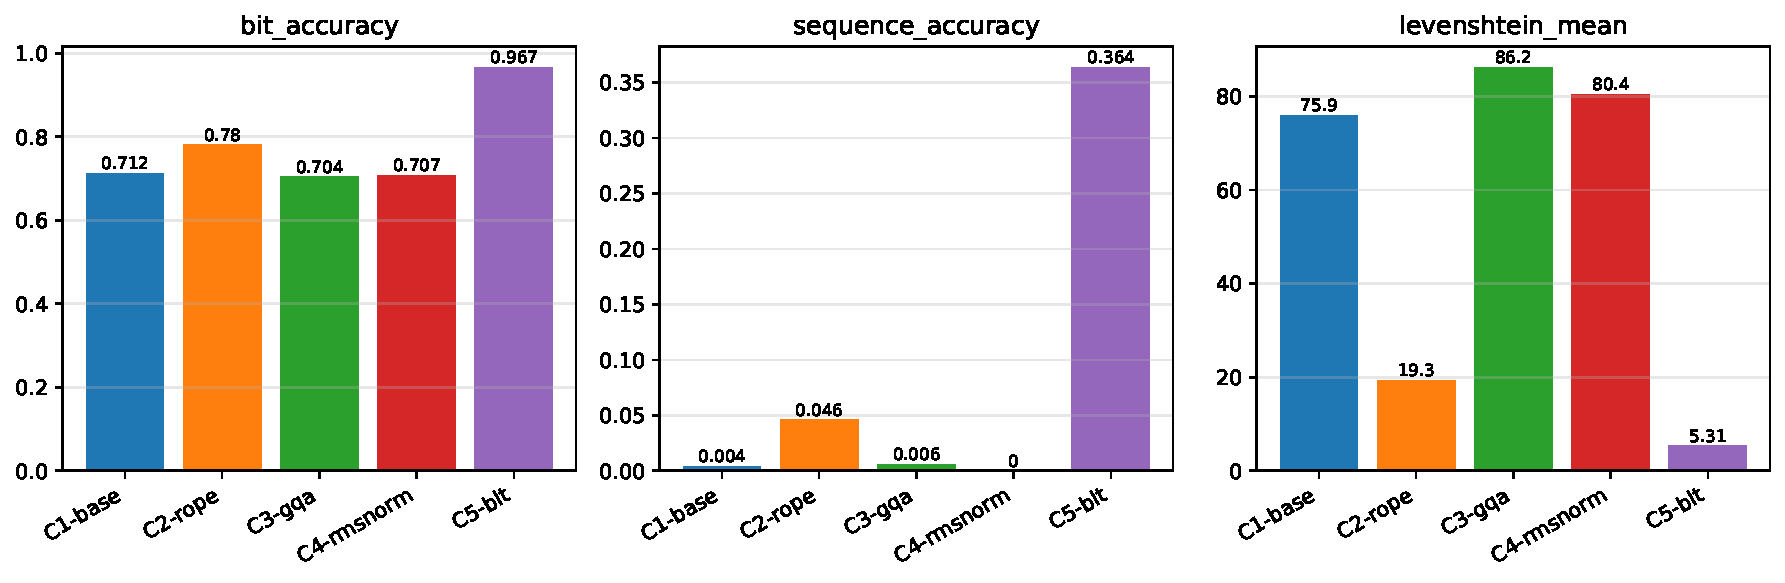
\includegraphics[width=0.8\linewidth]{../2023111026_assignment1/outputs/plots/metrics_all.pdf}
\caption{Overall test metrics across all five configurations.}
\end{figure}

\begin{figure}[!htb]
\centering
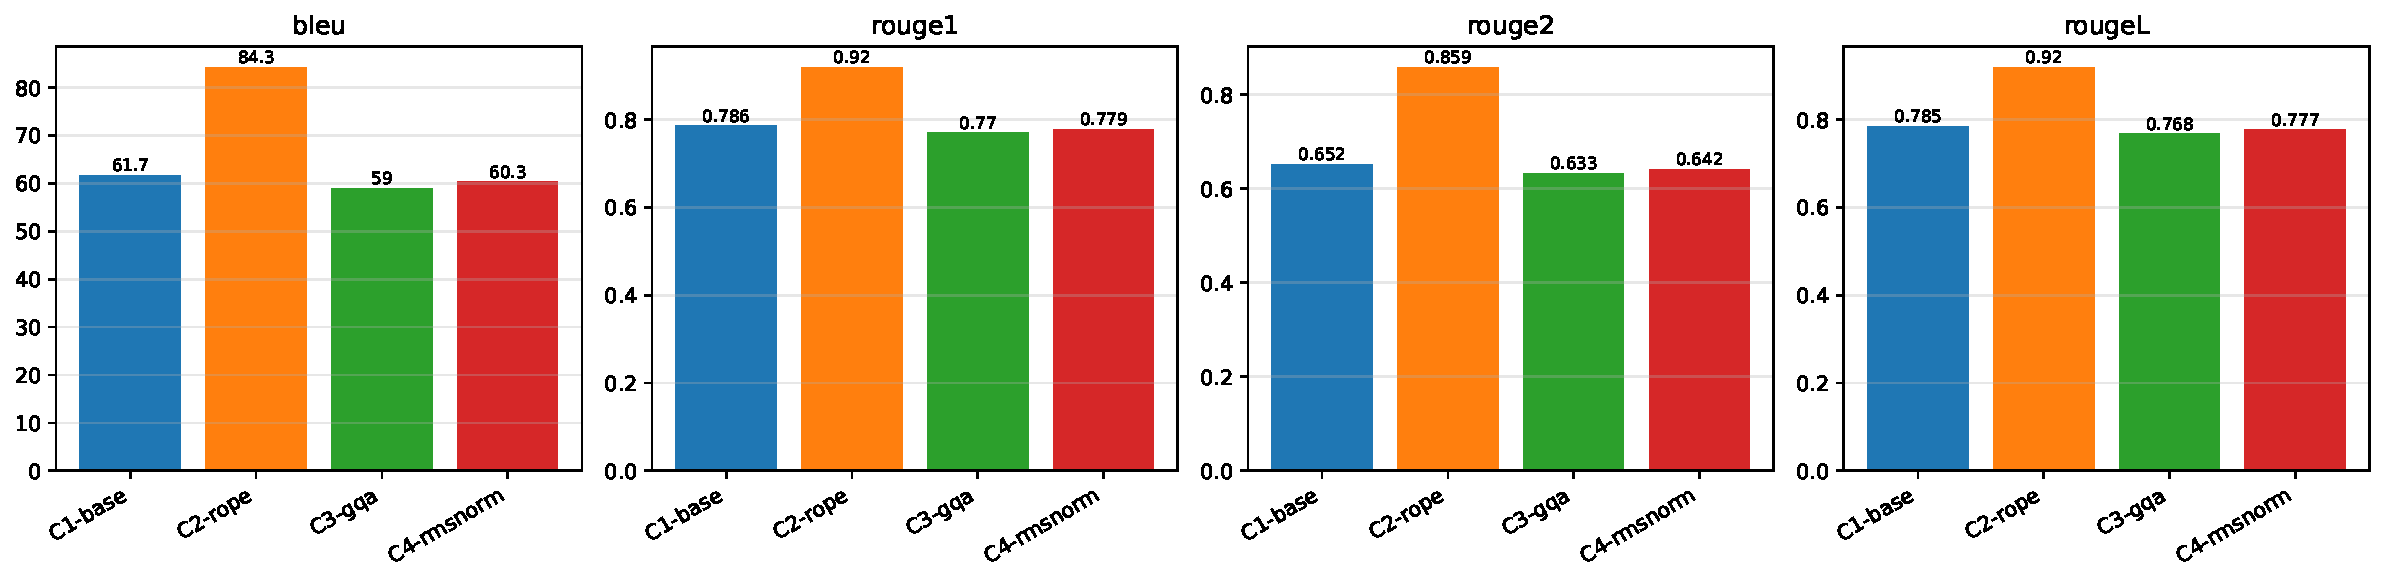
\includegraphics[width=0.8\linewidth]{../2023111026_assignment1/outputs/plots/metrics_bleu_rouge.pdf}
\caption{BLEU and ROUGE comparison for the tokenized configurations (C1--C4).}
\end{figure}

\begin{figure}[!htb]
\centering
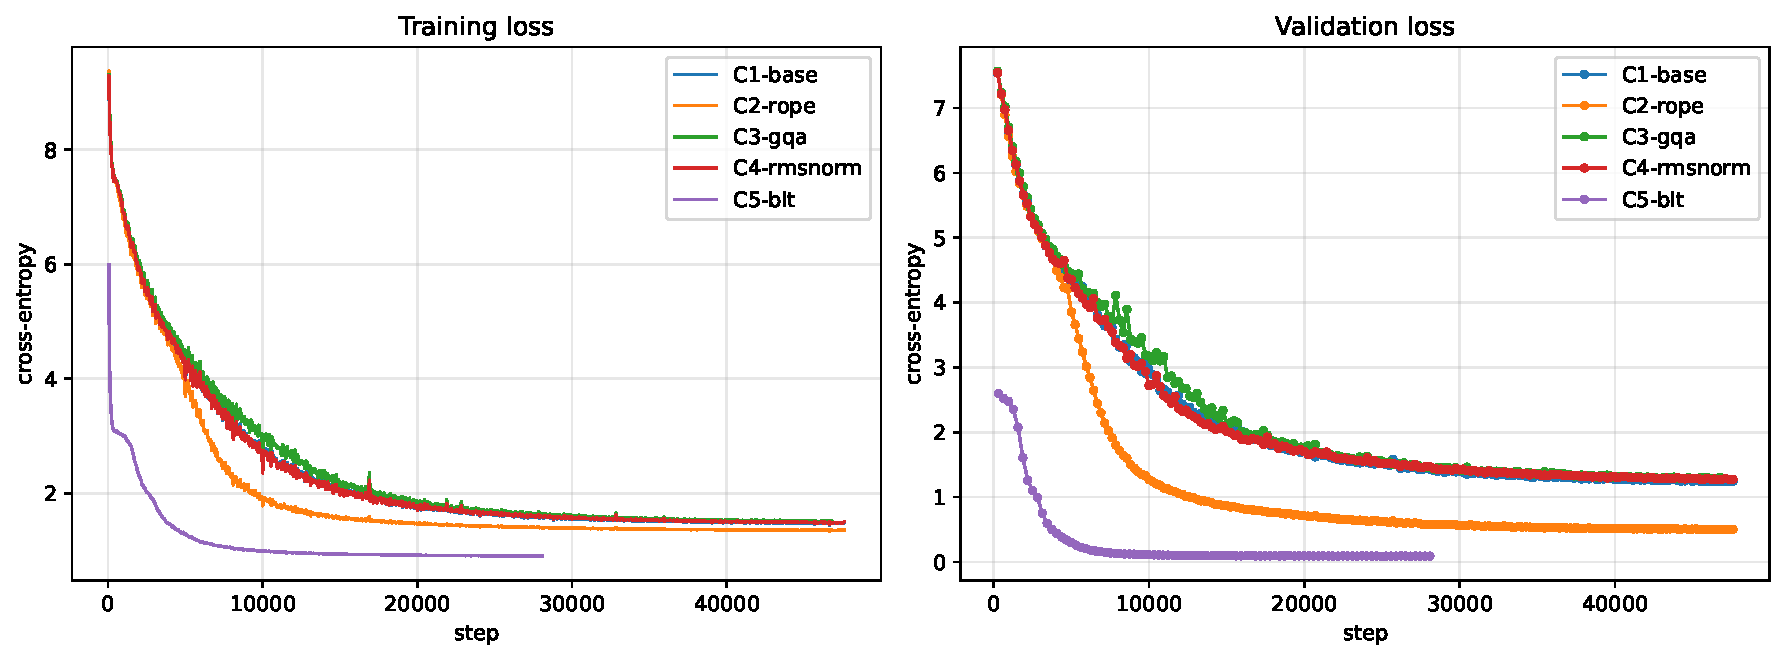
\includegraphics[width=0.8\linewidth]{../2023111026_assignment1/outputs/plots/loss_curves.pdf}
\caption{Training and validation loss for all configurations.}
\end{figure}

\subsection{C1: Baseline}

C1 is the baseline configuration, which uses sinusoidal absolute positional
encoding, multi-head attention, layer normalization, and standard subword
tokenization.

\subsection{C2: RoPE vs.\ sinusoidal absolute}

C2 replaces the sinusoidal absolute positional encoding of the base
Transformer~\cite{vaswani2017attention} with Rotary Positional Encoding
(RoPE)~\cite{su2021roformer}. While normal positional encoding turns the input into a fixed
embedding, and adds another vector which represents the position of the token,
RoPE doesn't have a separate positional embedding. Instead, it rotates the query
and key vectors based on their position. This can help the model to better
capture relative positions between tokens, in theory.

RoPE gives the best results out of all the tokenised models. Bit Accuracy increases from 
0.712 to 0.780, Levenshtein Distance drops from 75.91 to 19.30, BLEU increases from 61.74 
to 84.31, and ROUGE-1 from 0.786 to 0.920. C2 also has the lowest validation loss among 
the four tokenized models by a large margin, 0.497 compared with 1.238 for the baseline. 
It is also the only tokenised model that reconstructs a significant fraction of the test 
lines exactly, with a score of 4.6\% versus 0.4\% for the baseline.

I think this might be because in subword tokenisers the source and target are 
segmented independently. So the target tokens do not have a fixed alignment with the 
source tokens. The only constant thing is the relative positions between tokens, 
and RoPE captures this information effectively ($m - n$). This also explains why 
in my previous version, when the tokenisation was fixed width, and the mapping was 
really one to one, the scores were reversed and sinusoidal absolute positional encoding
performed slightly better than RoPE.

\subsection{C3: Grouped-Query vs.\ Multi-Head Attention}

In MHA, each attention head has its own query, key, and value matrices. In
GQA~\cite{ainslie2023gqa}, I split the 8 attention heads into 2 groups, so the 8 query heads share 2
key/value heads. Each key/value pair is shared across 4 query heads. This
reduces the key and value matrices from $256 \times 256$ to $256 \times 64$,
saving 98,304 weights and 384 bias terms per self-attention block. Across 8
blocks, this saves 789,504 parameters (8\%).

GQA is more useful in larger models, where the KV cache is big and can afford to
be reduced. In this case, the model is small, and the KV cache is already small,
so reducing it further only reduces accuracy. Bit Accuracy drops from 0.712 to
0.704, Levenshtein Distance rises from 75.91 to 86.24, and BLEU falls from 61.74
to 59.03. Its validation loss is the worst of the four at 1.281, against the
baseline's 1.238. Keys and values are the tensors that decide where
attention focusses, so reducing them from 8 heads to 2 reduces the diversity of the
matching the encoder can perform, and this task depends almost entirely on
pointing at the right source position. The saving in performance terms is not 
worth the drop in accuracy.

\subsection{C4: RMSNorm vs.\ LayerNorm}

This configuration changes the normalization layer from LayerNorm to
RMSNorm~\cite{zhang2019rmsnorm}.
LayerNorm subtracts the mean, divides by the standard deviation, then scales and
shifts by learned parameters. In RMSNorm, only the root mean square (RMS) of the
input is calculated, and the input is normalized using it. This reduces the
number of parameters in each normalization layer from 512 to 256, saving 256
parameters per layer. The model has 22 normalization sites in total (2 per
encoder layer, 3 per decoder layer, and a final norm on each stack), so this
saves 5,632 parameters (0.06\%).

Consequently, the performance of C4 is close to C1, with a Bit Accuracy of 0.707
(vs.\ 0.712) and Levenshtein Distance of 80.45 (vs.\ 75.91). The BLEU score is 60.30
compared to the baseline's 61.74, and the ROUGE scores are within about 0.01.
C4 was also the fastest configuration to train, at 684.0 samples/s against C1's 665.7, 
and used the least memory of the tokenized models at 2.85 GB against 3.00 GB. 
Dropping the mean-centering therefore bought a small speed and memory saving at no 
real cost in quality.

\subsection{C5: Token-free approach}

I replaced the original tokenizer with a simplified version of the Byte Latent
Transformer (BLT)~\cite{pagnoni2024blt}. C5 operates directly on the underlying bytes. 
Since the ciphertext is represented as a binary string, every 8 characters correspond to one
actual byte. I therefore group each sequence of 8 bits into a value between 0 and 255,
instead of treating each `0` or `1` character as a separate byte. This ensures that
the model operates on the encoded data itself instead of on its textual representation.
Thus, a 256-character chunk of the binary string corresponds to 256 source bytes.

The bytes are first mapped to embeddings and then processed by two local Transformer
layers. Each layer uses attention over windows of 128 positions. I determine patch
boundaries using entropy, following the approach in BLT, rather than splitting the
sequence at a fixed interval. Specifically, I estimate the entropy of the next byte
given the preceding context using an order-2 byte n-gram model with backoff. The n-gram
model is fitted only on the training split. A new patch is started when the predicted
next byte has entropy above a chosen threshold. I also impose a maximum patch length of
12 bytes so that a long sequence of predictable bytes cannot form an arbitrarily large patch.

I chose the entropy threshold from the training data. The threshold is the 75th percentile of 
the training entropy distribution, which gives 3.958 bits. This choice was important in practice.
In an earlier version, I used a threshold of 7 bits, but the maximum entropy observed in this
ciphertext was only 6.03 bits. As a result, the entropy condition was never triggered,
and every patch reached the 12-byte length limit. The resulting model was therefore
effectively doing fixed-width patching despite using the entropy-based procedure.
With the percentile-based threshold, 99.6\% of patch boundaries are triggered by entropy,
and the resulting patches range from 1 to 12 bytes, with an average length of 4.0 bytes.

Since the patches have different lengths, they cannot be combined using a simple reshape
operation. Instead, I compress each patch using cross-attention. A learned query attends
to all bytes within the corresponding patch, producing a fixed-size representation regardless
of the patch length while still allowing the representation to depend on the order of the bytes.

This approach performs far better than any tokenized configuration. It achieves
a Bit Accuracy of 0.967 and a Sequence Accuracy of 0.364, compared to 0.712 and
0.004 for C1, and its Levenshtein Distance is 5.31 against the baseline's 75.91.
Its validation loss, 0.088, is an order of magnitude below C1's 1.238, and more
than a third of test lines come back character-perfect where no tokenized model
manages even 5\%.

However, C5 is more expensive to train. It has 12.25M parameters compared to
9.68M for C1, and its throughput is much lower at 174.3 samples/s against 665.7.
Its training time per epoch rises from 17.2 seconds to 65.9 seconds, and peak GPU
memory from 3.00 GB to 4.92 GB. The extra cost comes from the byte-level local
encoder and decoder, which work on one position per cipher byte, and from the
cross-attention pooling that builds every patch. The global Transformer itself is
cheap, because patching has already shortened the sequence by about 4$\times$. C5
still processes more raw tokens per second than C1 (36.8k against 31.7k) while
handling far fewer sentences, which puts the cost in sequence length rather
than in the model being slow.

\begin{table}[!htb]
\centering
\small
\begin{tabular}{@{}lrrrrr@{}}
\toprule
Config & Params & Samples/s & Tokens/s & s/epoch & Peak GPU mem (GB) \\
\midrule
C1 (base) & 9.68M  & 665.7 & 31718 & 17.2 & 3.00 \\
C5 (BLT)  & 12.25M & 174.3 & 36814 & 65.9 & 4.92 \\
\bottomrule
\end{tabular}
\caption{Training efficiency, C1 vs.\ C5.}
\end{table}

\begin{figure}[!htb]
\centering
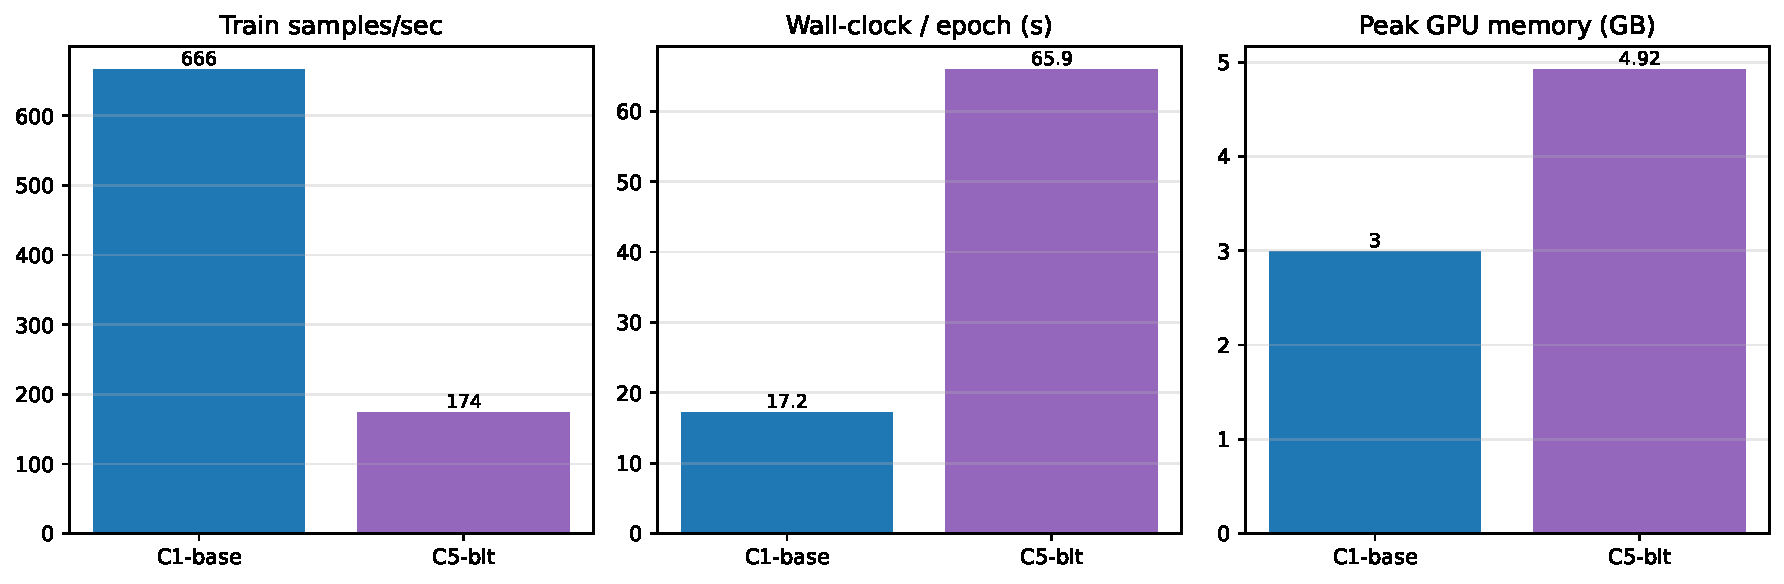
\includegraphics[width=0.78\linewidth]{../2023111026_assignment1/outputs/plots/c5_vs_c1_benchmark.pdf}
\caption{C1 vs.\ C5: throughput, wall-clock per epoch, and peak GPU memory.}
\end{figure}

\FloatBarrier

\begin{thebibliography}{9}\itemsep2pt

\bibitem{vaswani2017attention}
A.~Vaswani, N.~Shazeer, N.~Parmar, J.~Uszkoreit, L.~Jones, A.~N.~Gomez,
{\L}.~Kaiser, and I.~Polosukhin.
Attention Is All You Need.
In \emph{Advances in Neural Information Processing Systems (NeurIPS)}, 2017.

\bibitem{sennrich2016bpe}
R.~Sennrich, B.~Haddow, and A.~Birch.
Neural Machine Translation of Rare Words with Subword Units.
In \emph{Proceedings of the 54th Annual Meeting of the Association for
Computational Linguistics (ACL)}, 2016.

\bibitem{su2021roformer}
J.~Su, Y.~Lu, S.~Pan, A.~Murtadha, B.~Wen, and Y.~Liu.
RoFormer: Enhanced Transformer with Rotary Position Embedding.
\emph{arXiv preprint arXiv:2104.09864}, 2021.

\bibitem{ainslie2023gqa}
J.~Ainslie, J.~Lee-Thorp, M.~de~Jong, Y.~Zemlyanskiy, F.~Lebr\'on, and
S.~Sanghai.
GQA: Training Generalized Multi-Query Transformer Models from Multi-Head
Checkpoints.
In \emph{Proceedings of EMNLP}, 2023.

\bibitem{zhang2019rmsnorm}
B.~Zhang and R.~Sennrich.
Root Mean Square Layer Normalization.
In \emph{Advances in Neural Information Processing Systems (NeurIPS)}, 2019.

\bibitem{pagnoni2024blt}
A.~Pagnoni, R.~Pasunuru, P.~Rodriguez, J.~Nguyen, B.~Muller, M.~Li, C.~Zhou,
L.~Yu, J.~Weston, L.~Zettlemoyer, G.~Ghosh, M.~Lewis, A.~Holtzman, and S.~Iyer.
Byte Latent Transformer: Patches Scale Better Than Tokens.
\emph{arXiv preprint arXiv:2412.09871}, 2024.

\end{thebibliography}

\section*{Links}

\begin{itemize}\itemsep0pt
  \item Weights \& Biases project:
        \url{https://wandb.ai/arihanttr-iiit-hyderabad/anlp-a1}
  \item Hugging Face checkpoints:
        \url{https://huggingface.co/Arihant25/anlp-a1-transformer-ablations}
\end{itemize}

\end{document}
